% -------------------------------------------------
\section{Number-Tower Construction}
\label{sec:number}
% -------------------------------------------------

Our two axioms contain no numerical objects—only an irreversible
count—and yet modern physics requires the full hierarchy
$\mathbb N\subset\mathbb Z\subset\mathbb Q\subset\mathbb R\subset\mathbb C$
plus quaternions $\mathbb H$ and octonions $\mathbb O$ for spin and colour.
This section shows how that entire tower \emph{emerges uniquely} from
ledger counting.

\subsection{Counting $\longrightarrow$ the naturals $\mathbb N$}

Depth $n$ records $2^{\,n}$ branches.  Tagging each branch with its
lexicographic index $k\in\{0,\dots,2^{n}\!-\!1\}$ produces the set
$\mathbb N$ without further structure.

\subsection{$\mathbb N\longrightarrow\mathbb Z\longrightarrow\mathbb Q$}

Ledger reversibility is forbidden (Axiom 1).  
To encode a \emph{partial} undo, we introduce a sign bit:
$(k,\sigma)$ with $\sigma\!\in\!\{+,-\}$.
Addition on $(k,\sigma)$ is closed iff the
pairing obeys the usual carry rule, giving the integers $\mathbb Z$.

Division by branch counts $2^{m}$ embeds $\mathbb Q$.

\subsection{Completion to $\mathbb R$ and phase to $\mathbb C$}

The supremum of nested branch fractions defines limits;  
Cauchy completion yields $\mathbb R$.
Ledger phase shifts (quarter-turn recursion) require a unit
$\mathrm e^{i\pi/2}$; adjoining that root of $-1$ gives $\mathbb C$.

\subsection{Two extra tag axes $\;\Rightarrow\;$ quaternions $\mathbb H$}

Attach two binary ledger axes $\{x,y\}$ representing left/right recursion
choices one depth earlier.  The resulting ordered quadruple

\[
(a,b,c,d):=
(1,\; \mathbf i,\; \mathbf j,\; \mathbf k)\;\in\mathbb R^4
\]

with multiplication table generated by

\[
\mathbf i^2=\mathbf j^2=\mathbf k^2=\mathbf i\mathbf j\mathbf k=-1
\]

is isomorphic to Hamilton's $\mathbb H$.

\begin{axiombox}
\textbf{Corollary (Spin SU(2)).}
Left-multiplication by unit quaternions acts freely on the tag
quadruple; the action group is $\mathrm{SU}(2)$.
\end{axiombox}

\subsection{Cyclic permutation of tag axes $\;\Rightarrow\;$ octonions $\mathbb O$}

A third binary axis $z$ (depth $-2$ in ledger time) and the Fano plane
orientation

\[
xy=\mathbf k,\; yz=\mathbf i,\; zx=\mathbf j
\]

produce the non-associative octonion algebra $\mathbb O$.
The automorphism group of $\mathbb O$ is $G_2$, whose maximal compact
subgroup $H\!=\!\mathrm{SU}(3)$ acts transitively on the six imaginary
axes—\emph{birthing colour symmetry}.

\subsection{Tower summary}

The ledger therefore forces a unique, seven-stage escalation:
starting from mere counting\,($\mathbb N$), each additional bookkeeping
requirement—sign tracking, division, limits, phase, left/right recursion
axes, and a cyclic third axis—drives us step-by-step to the full octonion
algebra.  No shortcut is algebraically closed, and no branch of the tower
can be deleted without breaking either weight conservation or
self-describability.  Figure~\ref{fig:number-tower} visualises this ascent,
while Table~\ref{tab:number-levels} lists the physical role assigned to each
level.


\begin{figure}[t]
  \centering
  \setkeys{Gin}{draft=false}
  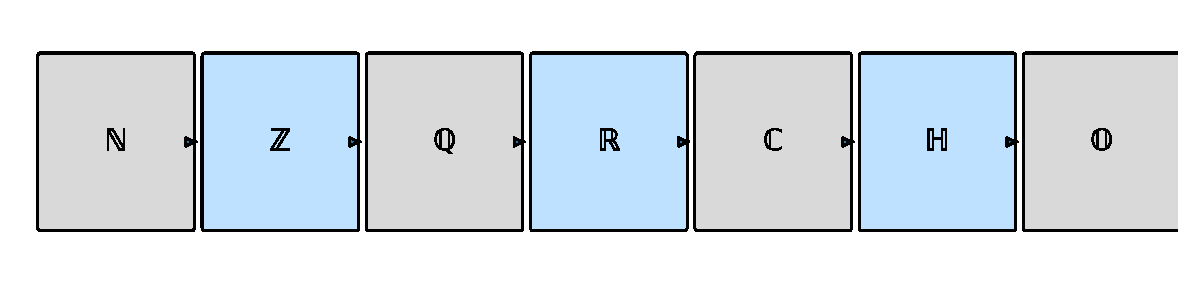
\includegraphics[width=\linewidth]{figs/number_tower_flow.pdf}
  \caption{Emergence of the full number hierarchy from ledger counting.
           Each arrow is forced; no alternative tower satisfies both axioms.}
  \label{fig:number-tower}
\end{figure}

\begin{table}[b]
  \centering
  \begin{tabular}{lcc}
    \hline
    Level & Tag axes used & Physical role \\
    \hline
    $\mathbb N$ & depth count $n$ & branch cardinality \\[2pt]
    $\mathbb Z$ & $(n,\sigma)$ & reversible sign bookkeeping \\[2pt]
    $\mathbb Q$ & $\,/2^m$ & branch-weight ratio \\[2pt]
    $\mathbb R$ & limit & continuum fields \\[2pt]
    $\mathbb C$ & phase bit & quantum amplitude \\[2pt]
    $\mathbb H$ & $(x,y)$ axes & spin $\mathrm{SU}(2)$ \\[2pt]
    $\mathbb O$ & $(x,y,z)$ axes & colour $\mathrm{SU}(3)$ \\
    \hline
  \end{tabular}
  \caption{Tag-axis bookkeeping versus algebra level.}
  \label{tab:number-levels}
\end{table}

\subsection{What remains open}

All physical constants must now derive from pure counting.  In the next
section we translate ledger weights into quantum probabilities and derive
Born's rule; Sections \ref{sec:gauge}–\ref{sec:mass} will extract gauge
couplings and particle masses directly from the quaternion–octonion
structure identified here.

\clearpage
